\documentclass[11pt]{article}
\pagestyle{empty}
\usepackage{multicol}

\usepackage{alltt}
\usepackage{tikz-qtree}
\usetikzlibrary{shadows,trees}
\usepackage{mathptmx}
\usepackage{graphicx}
%\newcommand{\includegraphics}{}



\newcommand{\lmb}{$\lambda$}
\newcommand{\bll}{\\\mbox{~~~~}$\bullet$}
\newcommand{\bk}[1]{$\langle${\bf #1}$\rangle$}

\newcommand{\lit}[1]{\mbox{\tt #1}}
\usepackage[listings]{tcolorbox}

\definecolor{codegreen}{rgb}{0,0.6,0}
\definecolor{codegray}{rgb}{0.5,0.5,0.5}
\definecolor{codepurple}{rgb}{0.58,0,0.82}
\definecolor{backcolour}{rgb}{0.95,0.95,0.92}

\lstdefinestyle{mystyle}{
    language=Lisp,
    backgroundcolor=\color{backcolour},   
    commentstyle=\color{codegreen},
    keywordstyle=\color{magenta},
    numberstyle=\tiny\color{codegray},
    stringstyle=\color{codepurple},
    basicstyle=\ttfamily\footnotesize,
    breakatwhitespace=false,         
    breaklines=true,                 
    captionpos=b,                    
    keepspaces=true,                 
    numbers=left,                    
    numbersep=5pt,                  
    showspaces=false,                
    showstringspaces=false,
    showtabs=false,                  
    tabsize=2,
    escapechar=|,
    frame=single
}

\lstset{style=mystyle}




\author{CSCI 312 Homework 4}
\title{Jabberwocks}

\begin{document}

\maketitle

\begin{multicols}{2}
\begin{itemize}
\item A {\bf jabberwock} is a borogove.
\item A {\bf borogove} is either:
  \begin{itemize}
  \item two jubjubs
  \item three borogoves
  \item a tove
  \end{itemize}
\item A {\bf jubjub} is either:
  \begin{itemize}
  \item a tove 
  \item two borogoves
  \end{itemize}
\item A {\bf tove} is two integers.  
\end{itemize}

\newcolumn
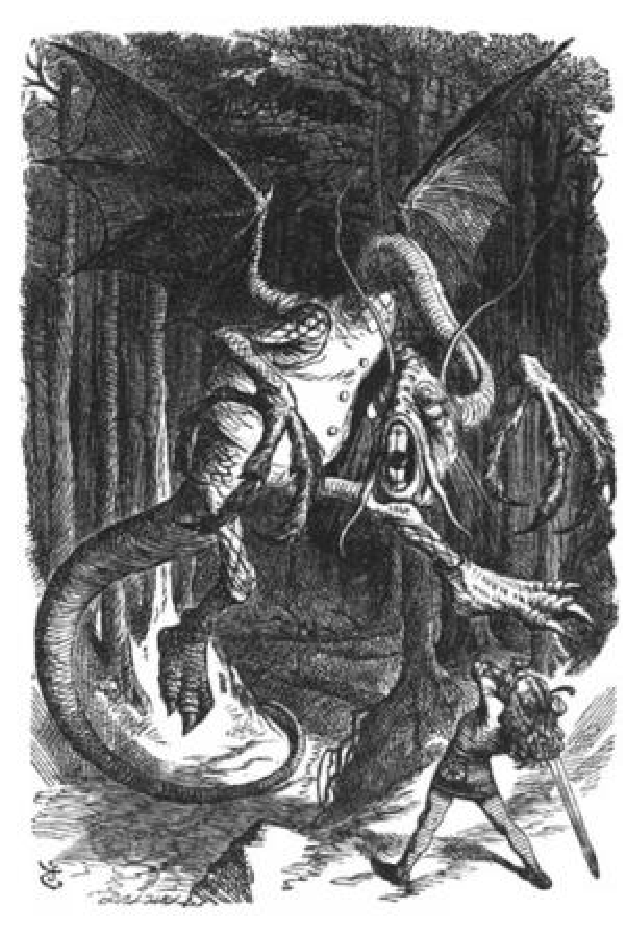
\includegraphics[width=0.5\textwidth]{jabberwocky}
\end{multicols}

Typical jabberwocks are shown below and above, right.

\hspace{-1cm}
\fbox{
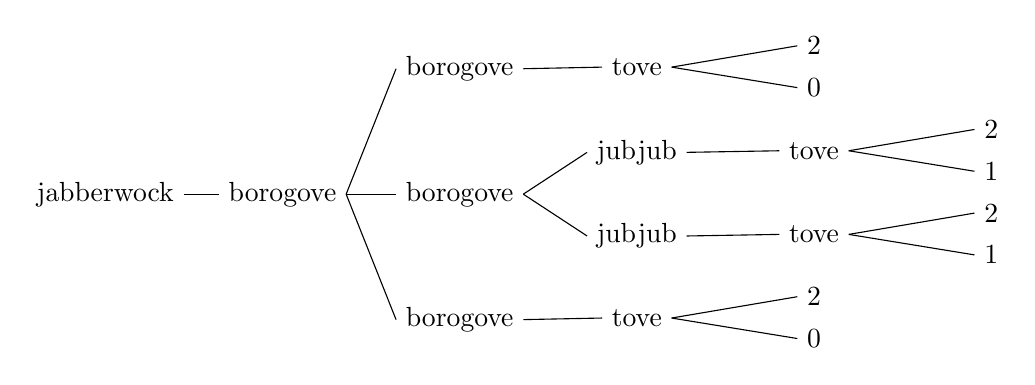
\begin{tikzpicture}[grow=right,level distance=2.25cm]
\Tree
  [.jabberwock
    [.borogove
      [.borogove
        [.tove
          [.0 ] [.2 ]
          ] ]
      [.borogove
        [.jubjub
          [.tove
            [.1 ]  [.2 ] ]]
        [.jubjub 
        [.tove
          [.1 ] [.2 ]
          ] ] ]
      [.borogove
        [.tove
          [.0 ]
          [.2 ]
          ] ] ] ]
\end{tikzpicture}
}
\begin{description}

\item[Types:]
Write a
definition of jabberwocks, borogoves, and toves
 in Racket language plai using {\tt define-type}.  

\item[Conversion to and from lists:]
Use your datatype to write a  procedure that converts
jabberwocks to lists.  For example:
\begin{lstlisting}
> (pretty-print (jabberwock-to-list test-case))
'(jabberwock
  (borogove
   ((borogove (tove 2 0))
    (borogove ((jubjub (tove 2 1)) (jubjub (tove 2 1))))
    (borogove (tove 2 0)))))
\end{lstlisting}
Note that the returned object is just a list of lists, symbols, and numbers.

Also write a procedure {\tt list-to-jabberwock} that takes a list, like the
one output by {\tt jabberwock-to-list}, and converts it into a genuine
jabberwock.

\item[Counting jubjubs and borogoves:]
 Also write a procedure {\tt fix-toves} that copies the
jabberwock, and replaces each pair of tove numbers with 
the number of borogoves and the number of jubjubs in the path
to the root.  This is true in the
jabberwock shown above.

\item[Test cases:]  Add enough unit tests to demonstrate
all features of your procedures.  These can be in the same
file or a separate file.


\item[Turn in:] Put all your files into a folder {\tt csci312lab04yourname},
zip it, and submit to canvas.


\end{description}

\end{document}

